\documentclass[aspectratio=169]{beamer}
\usepackage{hyperref,polski}
\usecolortheme{crane}
\usepackage{fontawesome5}

\definecolor{myorange}{RGB}{248,148,14}
\definecolor{jupyter}{HTML}{f37725}
\definecolor{myblue}{RGB}{107,167,220}
\definecolor{myyellow}{RGB}{255,231,132}
\definecolor{myred}{RGB}{247,148,143}
\definecolor{amber}{rgb}{1.0, 0.75, 0.0}
\definecolor{lightgrey}{HTML}{eeeeee}
\definecolor{grey}{HTML}{616262}
\definecolor{darkgrey}{HTML}{4e4e4e}

\setbeamercolor{item}{fg=amber}
\setbeamerfont{block title}{series=\bfseries}
\setbeamercolor{frametitle}{fg=white}

\beamertemplatenavigationsymbolsempty
\setbeamertemplate{footline}[frame number]

\useinnertheme{tcolorbox}

\makeatletter
\tcbset{
  boxrule=1pt,
  borderline={1pt}{0pt}{beamer@tcb@titlefg},
}
\makeatother

\newcommand{\faframetitle}[2]{\frametitle{{\color{white}#1}\quad {\color{white}#2}}}
\newcommand{\ourframe}{
    \setbeamercolor{block title}{bg=lightgrey}
    \setbeamercolor{block body}{bg=white, fg=structure}
}
\newcommand{\conclusionframe}{
    \setbeamercolor{block body}{bg=amber!20, fg=structure}
    \setbeamercolor{block title}{bg=structure, fg=amber!20}
}
\newcommand{\conclusions}[1]{
    \conclusionframe
    \centering
    \begin{block}{\centering \vspace{0.3em}\bf Conclusions\vspace{.3em}}
        {\begin{center}
            {#1}
        \end{center}}
    \end{block}}


\title{Continuous Integration with research notebooks:\\ on~maintaining reproducibility in atmospheric modeling}
\newcommand{\frametoctext}[1]{
{\addtocounter{framenumber}{-1}
     \begin{frame}
     \faframetitle{\faMapSigns}{What's next?}
        \begin{columns}[t]
        \begin{column}{.5\textwidth}
        \vspace{-3em}
        \bgroup
    \vskip1\baselineskip
    \fontsize{11}{25}\selectfont
    \tableofcontents[currentsection]
    \vskip0pt plus 1filll
  \egroup

        \end{column}
        \begin{column}{.37\textwidth}
        #1
        \end{column}
        \end{columns}
     \end{frame}
    % If you don't want them to affect the slide number
}}



\ourframe

\author{Agnieszka Żaba\texorpdfstring{\footnote{\texttt{azaba@agh.edu.pl}, AGH University of Krakow, Poland}}{}, Sylwester Arabas and \texttt{open-atmos} contributors}


  
\institute{UCAR Software Engineering Assembly Improving Scientific Software Conference\\\insertdate}
\date{Boulder, April 2025}
\setbeamertemplate{frametitle}[default][center]



\begin{document}

    \frame{
    \frametitle{
    {\color{structure}\small\insertinstitute}
        \vspace{2.5em}\\
        {\Large\inserttitle}\\
        {\color{structure}\normalsize\insertauthor}
        }
    \begin{columns}
        \begin{column}{.26\textwidth}
            
\includegraphics[width=\textwidth]{img/logo_zfs_en-crop}
        \end{column}
        \begin{column}{.2\textwidth}
            
\includegraphics[width=\textwidth]{img/AGH_logo.pdf} 
        \end{column}
        \begin{column}{.3\textwidth}
            
\includegraphics[width=\textwidth]{img/Atmos-logo-vert.pdf}
        \end{column}
    \end{columns}
    }

\begin{frame}
     \frametitle{Plan of this talk}
     
        \begin{columns}[t]
        \begin{column}{.5\textwidth}
        \vspace{-3em}
        \bgroup
    \vskip1\baselineskip
    \fontsize{11}{25}\selectfont
    \tableofcontents[]
    \vskip0pt plus 1filll
  \egroup

        \end{column}
        \begin{column}{.37\textwidth}
        
        \end{column}
        \end{columns}
        
     \end{frame}

\section{\texorpdfstring{\faLightbulb[regular]\quad}{} Why \ldots}
\subsection{\texorpdfstring{\qquad}{} \ldots reproducibility?}
    \frametoctext{} 
\frame{
    \faframetitle{\faLightbulb[regular]}{Why reproducibility?}
    

    \begin{columns}
    \begin{column}{.25\textwidth}
    \centering
        
\includegraphics[width=\textwidth]{img/gmd_cover.png}
    \end{column}
    \begin{column}{.75\textwidth}
    \Large
    \begin{block}{\href{https://gmd.copernicus.org/articles/12/2215/2019/}{Geoscientific Model Development (GMD) Guidelines}\footnote{\href{https://doi.org/10.5194/gmd-12-2215-2019}{DOI:10.5194/gmd-12-2215-2019 }}}
    \it
    \begin{itemize}
    \item ``necessary to have {access to all of the input data} (...)"
    \pause
    \item ``(...) all { model configuration} files are provided"
    \pause
    \item ``(...) no manual processing of the data"
    \pause
    \item ``All figures and tables must be { scientifically reproducible from the scripts}".
    \end{itemize}
    \end{block}
    \end{column}
    \end{columns}
}

% \Large Source code is necessary but not sufficient
\subsection{\texorpdfstring{\qquad \ldots}{} notebooks?}

\frame{
    \faframetitle{\faLightbulb[regular]}{Why notebooks?
    }
    
    \centering  
    \only<1-2>{\large{\color{structure}\bf ``Why Jupyter is data scientists’ computational notebook of choice"}\\
    \href{https://doi.org/10.1038/d41586-018-07196-1}{{\it Nature} 563 (toolbox): Perkel 2018}}
    \only<3>{\large{\color{structure}\bf Reactive, reproducible, collaborative: computational notebooks evolve}\\
     \href{https://doi.org/10.1038/d41586-021-01174-w}{{\it Nature} 593: Perkel 2021}\footnote{(J. F. Pimentel et al. in 2019 IEEE/ACM 16th International Conference on Mining Software Repositories (MSR) 507–517; IEEE, 2019)}}
    \vspace{2em}
    \Large
    \begin{columns}
        \begin{column}{.42\textwidth}
            \only<1-2>{
\includegraphics[width=\textwidth]{img/nature_2018.pdf}}
            \only<3>{
\includegraphics[width=1.1\textwidth]{img/nature2021}}
        \end{column}
        \begin{column}{.6\textwidth}
        \vspace{-1.5em}
        \begin{itemize}
        \item \it
            \only<1>{``We went from Jupyter notebooks not existing some six years ago to~in~essence everybody using them today''}
            \only<2>{``(...) difficult to organize code logically, break it into reusable modules and develop tests to ensure~the code is working properly''}
            \only<3>{ A 2019 study found that just {\bf 24\%} of 863,878 publicly available Jupyter notebooks on GitHub could be successfully {\bf re-executed}, and only {\bf4\%} produced {\bf the same results}}
        \end{itemize}
        \end{column}
    \end{columns}%Reactive, reproducible, collaborative: computational notebooks evolve
}
  



\section{ \texorpdfstring{\faCodeBranch\quad}{} open-atmos projects}
\frametoctext{
\begin{block}{Maintainability}
    Packages started over 5 years ago serve as good examples for discussion about maintainability.
\end{block}
}




% \frame{
%     \faframetitle{\faQuestion}{Questions}
% \framesubtitle{CI-integrated notebooks can help devs in maintaining test coverage, at the same time
% ensuring consistent/up-to-date tutorials for users}
        % \begin{block}{Research notebooks}
        % % Challenges: 
        % %     code compatibility, notebook sanity, result verification,
        % %     graphics
        % \end{block}
        % \begin{block}{Journals (e.g., GMD)} %Journal
        %     % enforce reproducibility against {\bf archived releases }
        % \end{block}
        % \begin{block}{can we do even better?!}%users and development
        %     % reproducibility is maintained also for {\bf future releases}! (with ongoing developments)
        % \end{block}
    % \centering
    % {\Large
    % How to approach {\bf\color{jupyter} maintainability} of {\bf\color{jupyter} reproducibility}\\ in projects with {\bf\color{jupyter} research notebooks}?\\
    % \vspace{.7em}
    % \pause
    % What  {\bf\color{jupyter} users} and {\bf\color{jupyter} devs} can gain?\\
    % \vspace{.7em}\pause
    % What is special in the {\bf\color{jupyter} atmospheric modeling}?}

% }


% NOTES
% algorithm from NCAR - PyMPDATA
  \frame{
  % \frametitle{\Large{\color{jupyter}\faCodeBranch}\, 
  %     \href{https://github.com/open-atmos/}{open-atmos} packages at PyPI
  %   }
  \faframetitle{\faCodeBranch}{Projects}
  \color{structure}
    \begin{columns}
        \begin{column}{.1\textwidth}
            
\includegraphics[width=\textwidth]{img/pysdm_logo.png}\\
        \end{column}
        \begin{column}{.85\textwidth}
            {\bf\color{myblue}PySDM} is a {\bf Pythonic high-performance} (multi-threaded CPU \& CUDA GPU) implementation of Monte-Carlo  {\bf Super-Droplet Method (SDM)} (Shima et al. 2009)
        \end{column}
    \end{columns}
    \pause
    \vspace{1em}
    \begin{columns}
        \begin{column}{.75\textwidth}
            {\bf\color{myblue}PyMPDATA} is a {\bf Numba-accelerated multi-threaded} Pythonic implementation of the NCAR-developed MPDATA algorithm used in geophysical fluid dynamics for solving advection-diffusion PDEs. 
        \end{column}
        \begin{column}{.1\textwidth}
            
\includegraphics[width=\textwidth]{img/logo_pympdata.png}
        \end{column}
    \end{columns}
    \pause
    \vspace{1em}
    \begin{columns}
        \begin{column}{.25\textwidth}
            
\includegraphics[width=\textwidth]{img/Atmos-logo-vert.pdf}
        \end{column}
        \begin{column}{.70\textwidth}
{\bf\color{myblue} {open-atmos-jupyter-utils}} provides utility routines for Jupyter notebooks for: automated testing; presenting {visuals}; pip-installation of external packages on Colab.
        \end{column}
    \end{columns}

  }
  

\section{\texorpdfstring{\faUsersCog \quad}{} Developers' perspective}
\frametoctext{
    \begin{block}{Devs gain}
        \begin{itemize}
            \item modularity and IoC
            \item dimensional analysis
            \item testing scenarios
            \item on-boarding new developers 
        \end{itemize}
    \end{block}
}



\frame{
{\huge\bf \vspace{2em}\\Inversion of Control\\\vspace{1em}}
\centering
{\Large prerequisite for reusability in atmospheric science\\
and for testing
% - IoC pomaga w testowaniu, ale nie w unit-testowaniu (bo IoC raczej dotyczy pracy z wieloma unitami), moze lepiej prerequisite for reusability in atmos. sci. (and for testing, and for...);
}
}

\begin{frame}[fragile]
    \faframetitle{\faUsersCog}{Atmospheric science:
    \\parameterizations and simulation flow control}
    
    
% we want to go for classics - title of Bolins book, IPCC directo
    \centering
    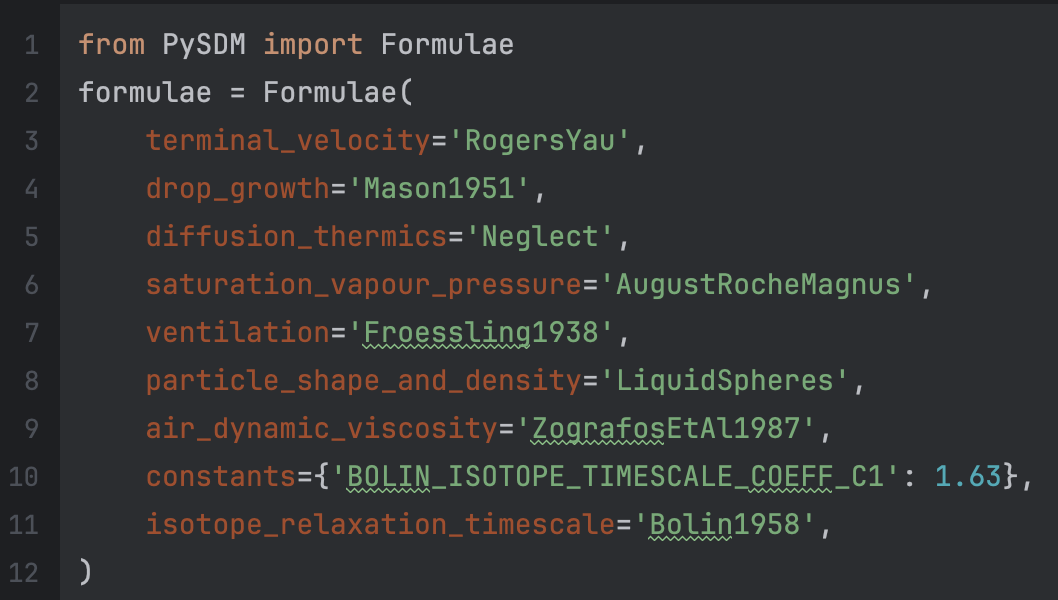
\includegraphics[width=.7\textwidth]{img/Bolin_formula.png}
    
    % PySDM formulae
    % example implementation  (with formulae variant choices from user scope, enabling each maintained notebook to use different constants, and physics formulae, in atmospherics modeling often there is no grand truth)
    % \centering
    % Modularity and inversion of control
\end{frame}

\frame{
    \faframetitle{ \faUsersCog}{Dimensional analysis of the code}
    
    \centering
    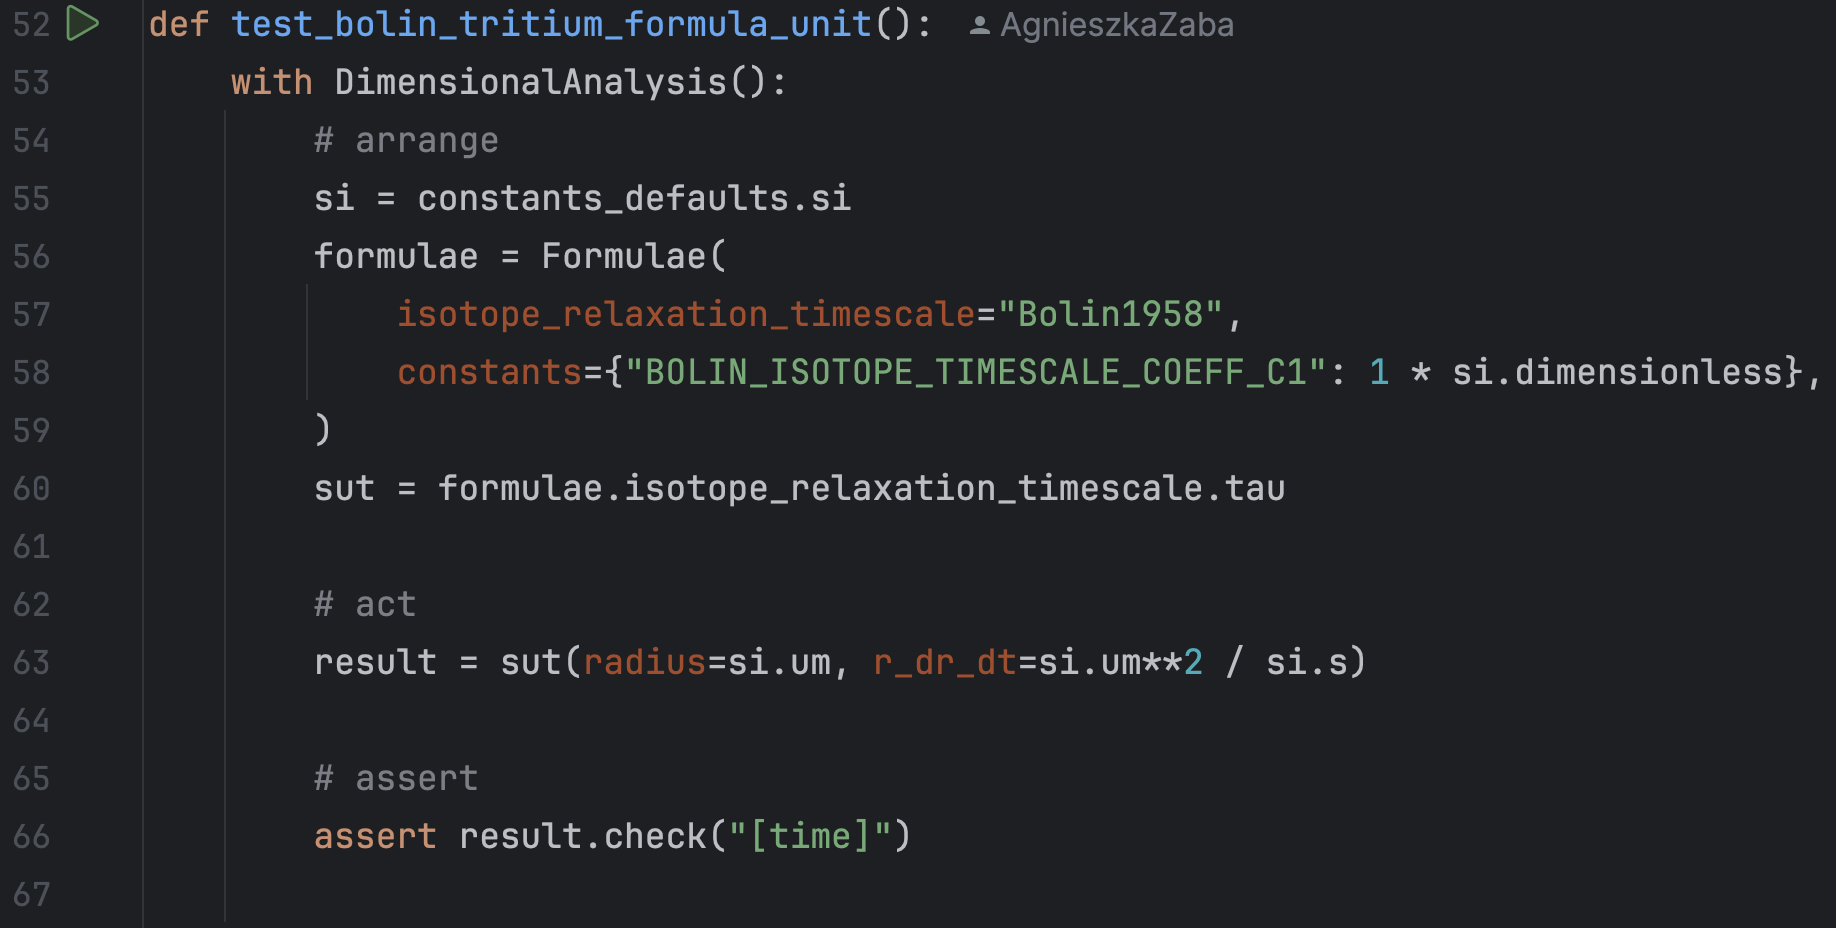
\includegraphics[width=.8\textwidth]{img/Bolin_test.png}
    }
    
    
\frame{
    \faframetitle{\faUsersCog}{Notebooks as a source of test (edge) cases!}
    \centering

        
        \begin{columns}
        \begin{column}{.45\textwidth}
        \centering
        {\Large\bf pip install open-atmos-jupyter-utils}
            \begin{block}{notebook\_vars()}
        
          \begin{itemize}
                \item executes unmodified notebook code for automated testing
                \item run-once/multiple asserts\\ ~~(using pytest fixture)
            \end{itemize}  
        \end{block}
         
            
\includegraphics[width=.2\textwidth]{img/pytest1.png}
            
\includegraphics[width=.35\textwidth]{img/Atmos-logo-vert.pdf}
        
        \end{column}
        
        \begin{column}{.55\textwidth}
        \vspace{.2em}
        
            \only<1>{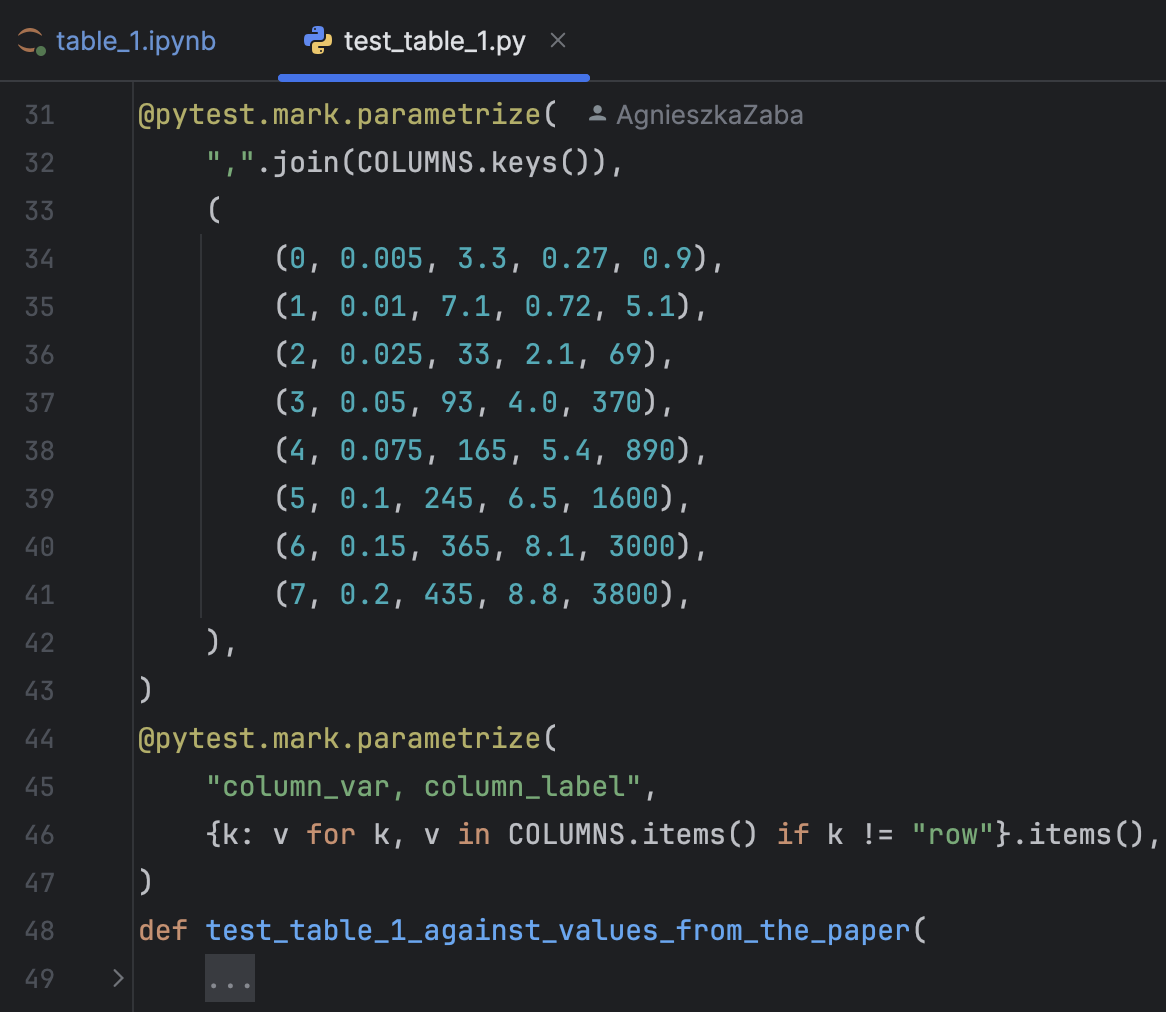
\includegraphics[width=\textwidth]{img/test_table.png}}
            % \only<2>{\pgfimage[width=.9\textwidth]{img/s_shot_test}}
        \end{column}
        \end{columns}
}


\frame{
\faframetitle{\faUsersCog}{\href{https://drive.google.com/file/d/1hJEXZ3XOcUsxQU0KhD3hqbGT4KLclBQe/view?usp=share_link}{Developers' perspective --- DEMO}}
\begin{columns}
    \begin{column}{.3\textwidth}
        
\includegraphics[height=.6\textheight]{img/pysdm_logo.png}
    \end{column}
    \begin{column}{.5\textwidth}
        \begin{itemize}
            \item IoC - formulae chosen by user
            \item dimensional analysis can be done because of that
            \item unit tests outside of notebooks
            \item on-boarding new developers
        \end{itemize}
    \end{column}
\end{columns}
}

\section{\texorpdfstring{\faUsers \quad}{} Users' perspective}
\frametoctext{
    \begin{block}{Users gain}
        \begin{itemize}
            \item self-contained notebooks ready to run
            \item compliance with journal requirements
            \item maintainable visuals in research-notebooks
        \end{itemize}
    \end{block}
}


\frame{
    \faframetitle{\faUsers}{Maintainable visuals in research-notebooks}
    \begin{columns}[t]
        \begin{column}{.42\textwidth}{\bf
        import open\_atmos\_jupyter\_utils}
        \centering
        \only<1->{
            \begin{block}{\bf show\_plot()}
              \begin{itemize}
                  \item gives SVG inline graphics
                  \item adds save-SVG/PDF buttons
                  \item Google-Drive link on Colab
                  \item renders OK on GitHub
              \end{itemize}
            \end{block}
        }
        \only<2->{
            \begin{block}{\bf show\_anim()}
              \begin{itemize}
                  \item uses matplotlib \& imageio
                  \item GIF$\leadsto$base64$\leadsto$.ipynb JSON
                  \item save-as-GIF button +Colab
                  \item renders OK on GitHub
              \end{itemize}
            \end{block}
        }
        
        \end{column}
        \begin{column}{.46\textwidth}
        {
              \only<1>{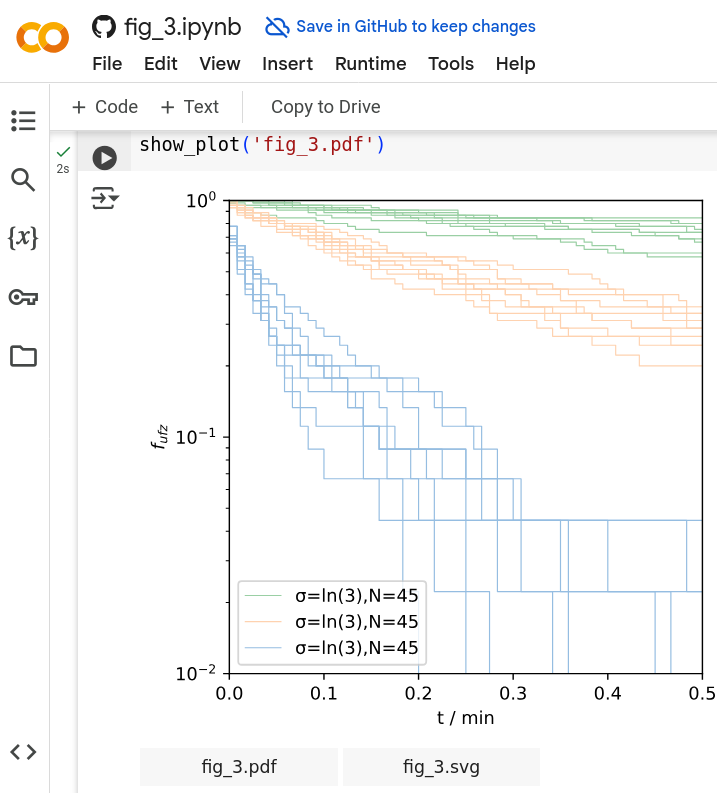
\includegraphics[width=\linewidth]{img/sshot_colab} }
              \only<2>{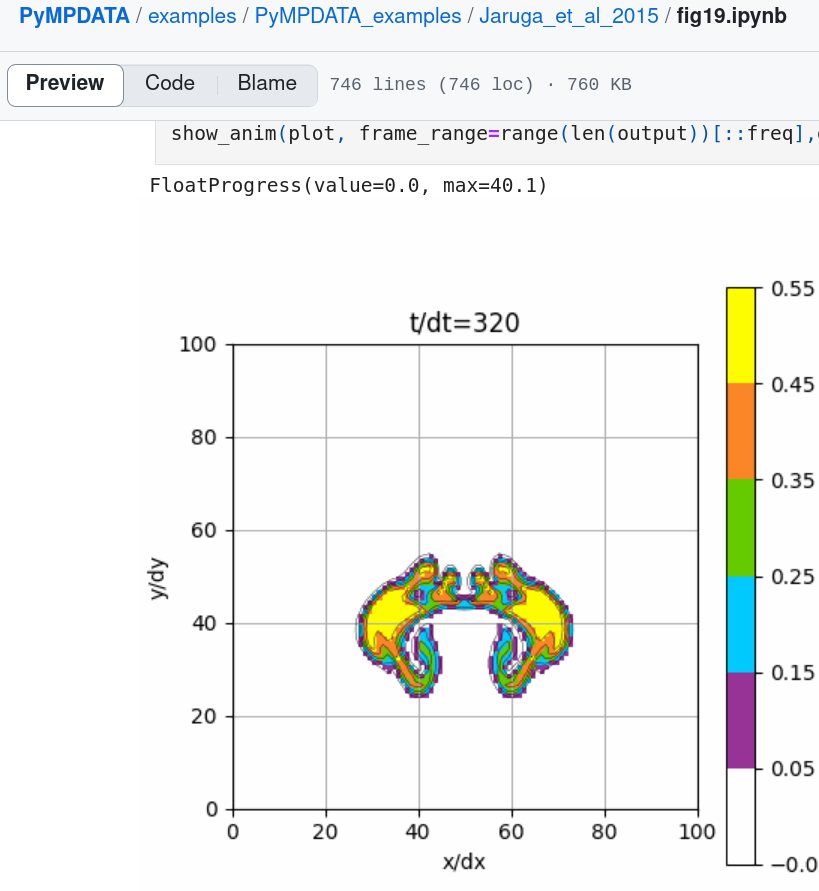
\includegraphics[width=\linewidth]{img/sshot_anim}}
        }
        \end{column}
    \end{columns}
}

\frame{
    \faframetitle{\faUsers}{\href{https://drive.google.com/file/d/1uhyqPQnh9HRF59SbfNI42iosUQBcVZ_5/view?usp=share_link}{Users' perspective -- DEMO}}
        \begin{columns}
            \begin{column}{.3\textwidth}
                
\includegraphics[width=\textwidth]{img/logo_pympdata.png}
            \end{column}
            \begin{column}{.6\textwidth}
        \begin{itemize}
                    \item notebooks are great for tutorials, but only if kept up-to-date with ongoing development (with CI automation!)
                    \item paper-author (compliance with journal requirements) / paper-reviewer perspectives
                    \item maintainable visuals in research-notebooks
                \end{itemize}
            \end{column}
        \end{columns}
      
      %DEMO (documentation -> Colab -> animation + graphics
}


\section{\texorpdfstring{\faList \quad}{} Summary}
\frametoctext{}

\frame{
\faframetitle{\faClipboardCheck}{Take home messages}% \faHome \, \faClipboardList}
\large
%TODO make them to be remeberable? 

\begin{block}{\centering \Large Essential integration}
\centering
     Research notebooks + automated testing workflows
\end{block}
\pause
\begin{block}{\centering \Large Modularity and IoC}
    \centering Benefits for users, developers and on-boarding new contributors
\end{block}
\pause
\begin{block}{\centering \Large Generated and embedded visuals}
\centering
force reproducibility, easier to maintain
\end{block}
\pause
\begin{block}{\centering\Large Maintenance of research-result reproducibility}
\centering Supports ongoing project development
\end{block}

}

\frame{
\faframetitle{\faGlobeAmericas}{Acknowledgments }
\centering

\includegraphics[height=.2\textheight]{img/Atmos-logo-vert}\\

\includegraphics[width=.6\textwidth]{img/logo-poziom-en-crop.pdf} \\

\includegraphics[height=.2\textheight]{img/agh_idub_en_cmyk.pdf}

\includegraphics[height=.2\textheight]{img/ncar_mmm_logo.jpg}

\vspace{4em}
\large
Thank you for your attention!
}








\end{document}

            \conclusions{CI-integrated notebooks can help devs in maintaining test coverage, at the same time ensuring consistent/up-to-date tutorials for users\\new}